\section{Predecessor branch validation (supplement)}
\label{sec:predecessor-branches}

This supplement preserves, nearly intact, the historical Model~A /
Model~B2 branch-construction and branch-separation validation. It is
audit evidence, not part of the main results path. Historical Model~A
($H_{0}=73.21$,
\path{runs/cmb_reconstruction/frozen/MODEL_A_FINAL.json}) was one
attempted physical realization of distance-preferred behavior; it fails
full Planck and is \textbf{not} the endpoint R ($H_{0}=72.80$,
\path{runs/cmb_bridge/r3/smooth_lowz_history.npz}). Historical Model~B2
provided the lineage from which the C1 CMB-compatible background was
obtained. See the endpoint identity contract
(\path{paper/evidence/endpoint_identity_contract.json}).

\subsection{Historical CMB-branch construction}
\label{sec:b2branch}

The historical distance-branch construction achieved its late-time
distance fit, but that result alone cannot address the Hubble tension,
because the tension is a disagreement \textit{between} datasets. This
subsection constructs the other side of the historical comparison: a
CMB-calibrated branch, called Model~B2, built without inheriting
anything from the distance-branch machinery (claim B2-SPLIT).

Construction proceeded in staged layers, each frozen before the next
opened. Stage~0 tuned a flat $\Lambda$CDM background to Planck
TT/TE/EE only (six parameters:
$H_{0}$, $\omega_{b}h^{2}$, $\omega_{c}h^{2}$, $\tau$, $A_{s}$,
$n_{s}$). Layer~1 tested early-expansion features around that
background: only zero amplitude survived, so no early feature entered
the branch. Layer~2 added primordial freedom (tilt and running);
a mild running was preferred. Layer~3 opened perturbation freedom
beyond GR (coupling rescaling): it worsened the fit at every tested
point, so GR perturbations were retained with zero additional freedom.
The selected B2 cosmologies therefore carry
$\MXXVIIIBTwoKB$ fitted parameters against $\MXXVIIIBTwoKA$ on the
distance branch (claim B2-COMPLEXITY), and its spectra reproduce
through an independent Cobaya-theory pipeline path as well as the
direct Boltzmann evaluation (claim B2-REPRODUCTION; Appendix~F
records the channel-activation checks that make this comparison
honest).

Model~B2 is thus ordinary $\Lambda$CDM with running and GR
perturbations, calibrated to the CMB. It is not a patched distance
model: no distance-branch parameter, table, or likelihood entered its
construction. Its low-redshift predictions (DESI, supernovae, ladder
anchor) are post-hoc projections, reported in
Supplement~\ref{sec:separation} as the price of CMB compatibility.

\subsection{Historical branch separation}
\label{sec:separation}

With both historical branches frozen, the comparison is purely
descriptive: no further fitting, no reweighting. Model~A is the
historical distance-calibrated expansion history
($H_{0} = \MXXVIIIBTwoHZeroA$\kmsMpc{}); Model~B2 is the
CMB-calibrated acoustic/primordial history
($H_{0} = \MXXVIIIBTwoHZeroB$\kmsMpc{}). Table~\ref{tab:ab-comparison} lists
the sector budgets side by side, and
Figs.~\ref{fig:b2-hz}--\ref{fig:b2-budget} show the four faces of the
separation (claim B2-SPLIT).

\begin{table}[!htbp]
  \centering
  \caption{Distance-calibrated branch (A) versus CMB-calibrated branch
  (B2): sector $\chi^{2}$ budgets and calibration scales from frozen
  evidence.}
  \label{tab:ab-comparison}
  \begin{tabular}{lrrr}
\toprule
Sector & Model A (distance) & Model B2 (CMB) & $\Delta$ (B2$-$A) \\
\midrule
$H_{0}$ [km\,s$^{-1}$\,Mpc$^{-1}$] & 73.21 & 67.99 & -- \\
$r_{\mathrm{drag}}$ [Mpc] & 135.48 & 147.15 & +11.66 \\
DESI DR2 $\chi^{2}$ & 6.1 & 18.0 & +11.87 \\
Pantheon+SH0ES $\chi^{2}$ (profiled $M$) & 1448.5 & 1490.2 & +41.70 \\
DESI+SN $\chi^{2}$ & 1454.5 & 1508.1 & +53.57 \\
SHOES-ladder $\chi^{2}$ & 0.0 & 25.0 & +25.00 \\
Planck low-$\ell$ TT $\chi^{2}$ & excluded (non-finite) & 22.1 & -- \\
Planck low-$\ell$ EE $\chi^{2}$ & 409.8 & 396.1 & -13.71 \\
Planck high-$\ell$ TTTEEE $\chi^{2}$ & 13169.8 & 583.8 & -12586.0 \\
Fitted parameters (excl. profiled $M$) & 21 & 7 & -- \\
\bottomrule
\end{tabular}

{\small Model A: M28-A distance-calibrated expansion history ($H_{0,\mathrm{phys}}$ from the frozen background table). Model B2: independent CMB-calibrated $\Lambda$CDM${}+{}$running branch with GR perturbations (no M28 inheritance). $\Delta\chi^{2}$ convention follows the frozen likelihood budget: negative favors B2. SN $M$ analytically profiled in both branches.\par}

\end{table}

\subsubsection{Expansion histories}

Figure~\ref{fig:b2-hz} compares $H_{A}(z)$ and $H_{B}(z)$ with their
fractional difference. The branches differ at all redshifts shown,
with maximum fractional separation $\MXXVIIIBTwoDHMax$ near $z \approx
3.8$ where the distance branch carries its early-epoch feature; at
$z = 0$ the offset is the familiar $H_{0}$ difference,
$\MXXVIIIBTwoHZeroA$ versus $\MXXVIIIBTwoHZeroB$\kmsMpc{}.

\begin{figure}[!htbp]
  \centering
  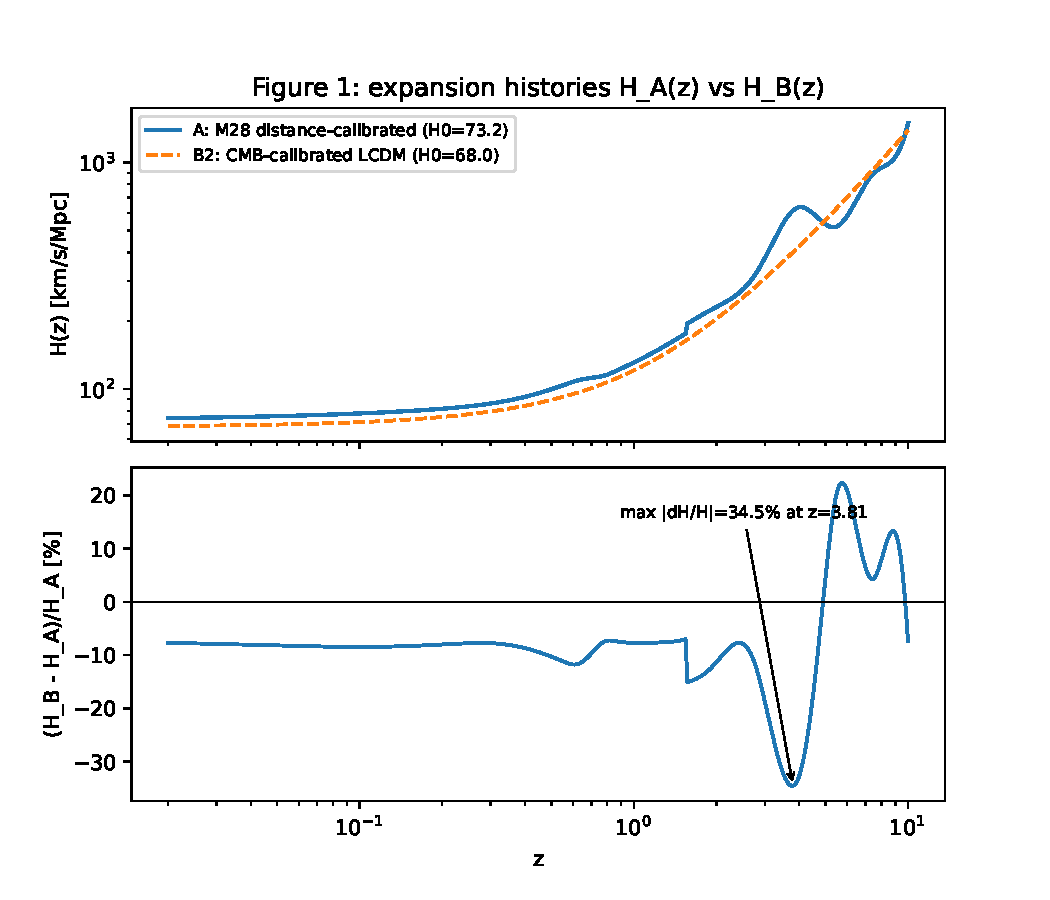
\includegraphics[width=0.85\linewidth]{figures/b2/fig1_expansion.pdf}
  \caption{Expansion histories $H_{A}(z)$ (distance branch) and
  $H_{B}(z)$ (CMB branch) with fractional difference
  $(H_{B}-H_{A})/H_{A}$. The separation spans low and high redshift.}
  \label{fig:b2-hz}
\end{figure}

\subsubsection{Acoustic calibration}

Figure~\ref{fig:b2-rd} shows the sound-horizon scales:
$r_{\mathrm{drag}} = \MXXVIIIBTwoRdA$~Mpc for branch~A versus
$\MXXVIIIBTwoRdB$~Mpc for branch~B2, a difference of
$\MXXVIIIBTwoDeltaRd$~Mpc. This is the most intuitive physical face of
the split: the two calibrations disagree on the size of the standard
ruler itself, so no late-time re-mapping can bring them together
without moving the early-universe physics that sets the ruler.

\begin{figure}[!htbp]
  \centering
  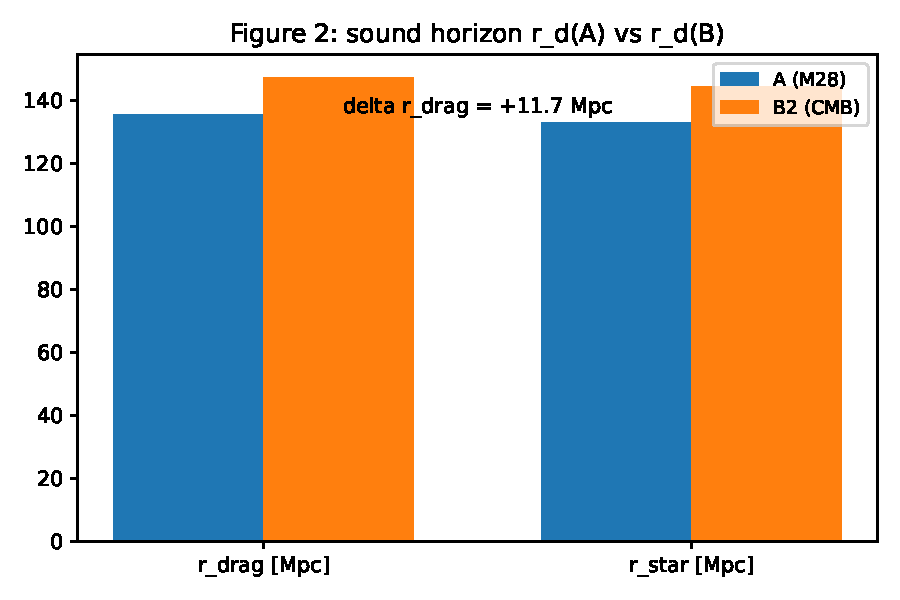
\includegraphics[width=0.85\linewidth]{figures/b2/fig2_sound_horizon.pdf}
  \caption{Sound-horizon calibration:
  $r_{\mathrm{drag}} = \MXXVIIIBTwoRdA$~Mpc (A) versus
  $\MXXVIIIBTwoRdB$~Mpc (B2).}
  \label{fig:b2-rd}
\end{figure}

\subsubsection{CMB spectra}

Figure~\ref{fig:b2-tt} shows binned Planck TT residuals for both
branches. Branch~B2 tracks the acoustic structure
(high-$\ell$ $\chi^{2} = \MXXVIIIBTwoHighlB$, low-$\ell$ TT
$\chi^{2} = \MXXVIIIBTwoLowTtB$); branch~A misses peak heights and phases
(high-$\ell$ $\chi^{2} = \MXXVIIIBTwoHighlA$, low-$\ell$ TT non-finite).
The CMB therefore excludes the historical distance branch outright rather than
merely disfavoring it.

\begin{figure}[!htbp]
  \centering
  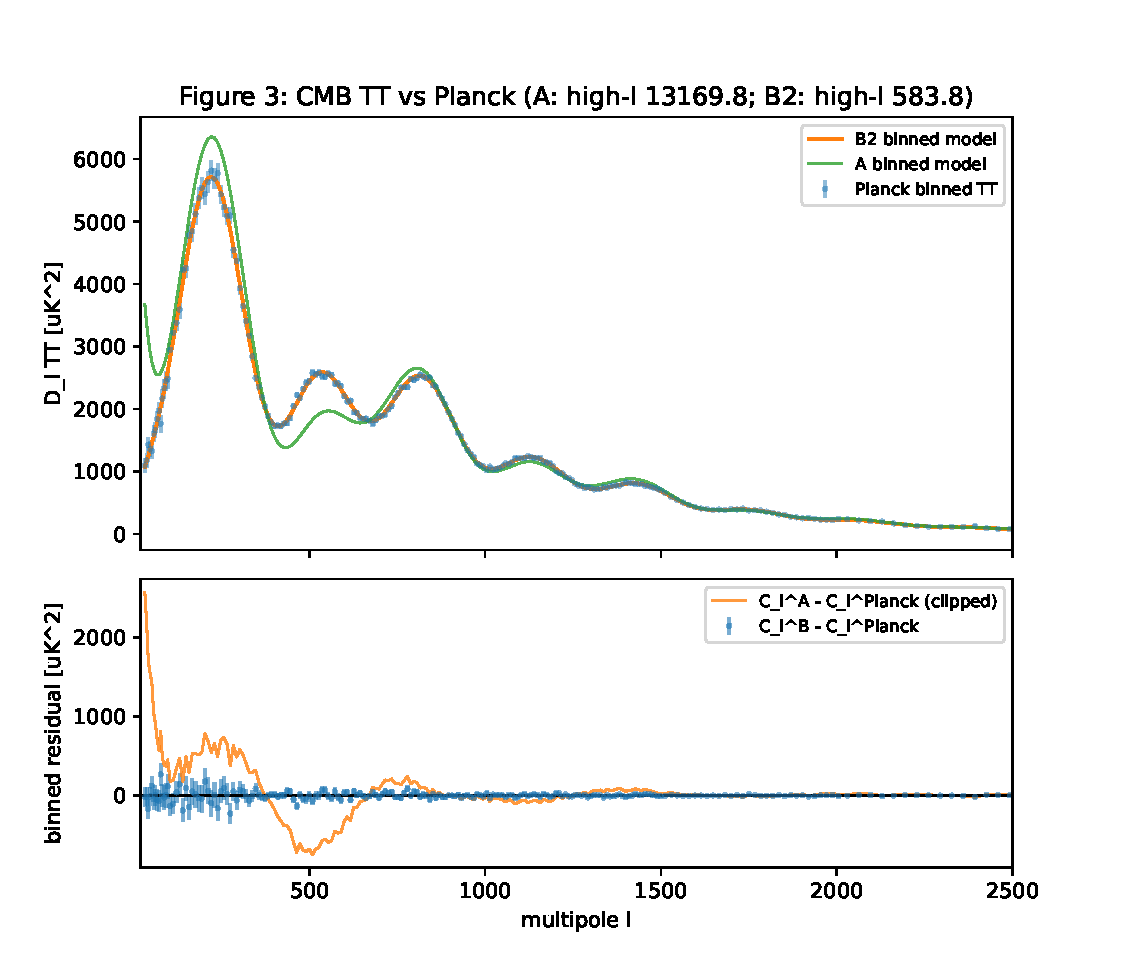
\includegraphics[width=0.85\linewidth]{figures/b2/fig3_cmb_residuals.pdf}
  \caption{Binned Planck TT residuals
  $C_{\ell}^{\mathrm{branch}} - C_{\ell}^{\mathrm{Planck}}$ for both
  branches. B2 tracks the acoustic peaks; A misses their heights and
  phases and is excluded at low $\ell$.}
  \label{fig:b2-tt}
\end{figure}

\subsubsection{Likelihood budget}

Figure~\ref{fig:b2-budget} stacks the sector budgets. Branch~A pays
almost entirely in the CMB column; branch~B2 pays in the
distance/ladder columns (DESI+SN
$\MXXVIIIBTwoDesiSnA$ versus $\MXXVIIIBTwoDesiSnB$; ladder
$\MXXVIIIBTwoLadderA$ versus $\MXXVIIIBTwoLadderB$). Neither branch fits
everything (claims B2-RESOLUTION, B2-MG, B2-LCDM-FAILURE record what
is \textit{not} claimed). The tension, within the tested model
classes, is this mismatch between a distance-calibrated expansion
history and a CMB-calibrated acoustic/primordial history.

\begin{figure}[!htbp]
  \centering
  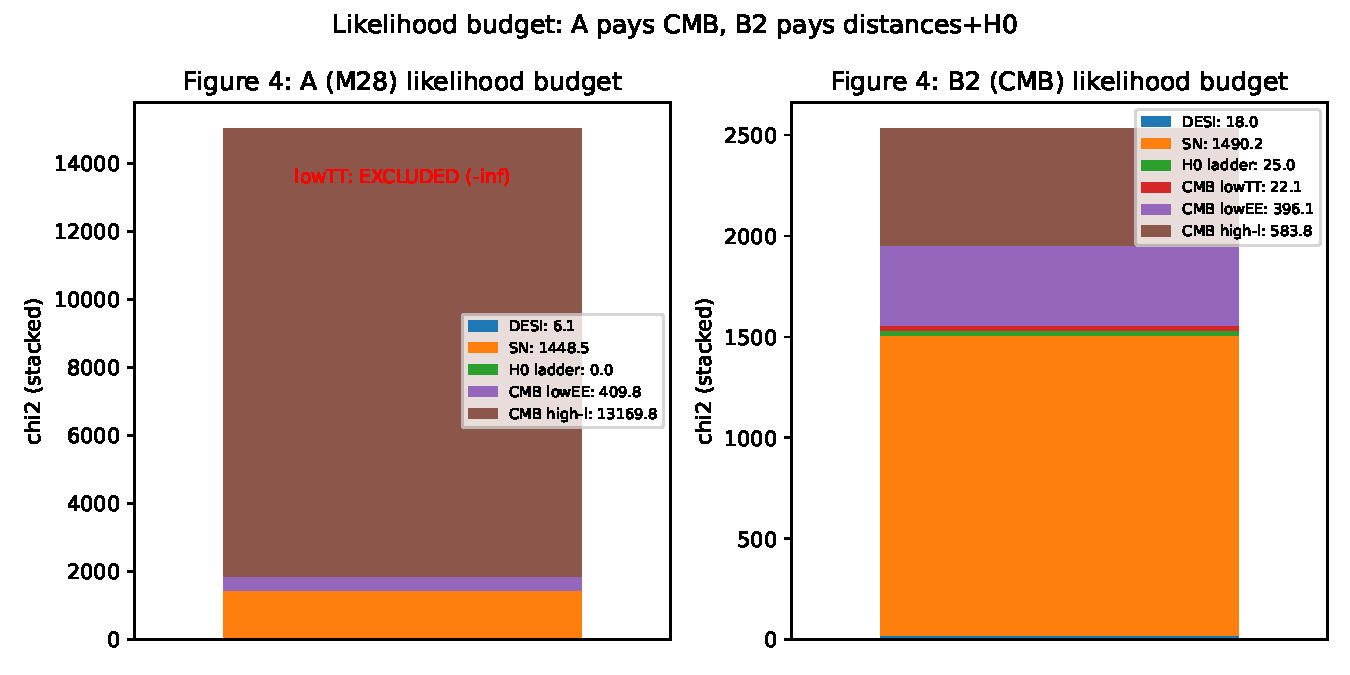
\includegraphics[width=0.85\linewidth]{figures/b2/fig4_likelihood_budget.pdf}
  \caption{Stacked sector $\chi^{2}$ budgets. A pays the CMB penalty;
  B2 pays the distance/ladder penalty. The low-$\ell$ TT entry excludes
  branch~A (non-finite).}
  \label{fig:b2-budget}
\end{figure}
\FloatBarrier
